\let\negmedspace\undefined
\let\negthickspace\undefined
\documentclass[journal]{IEEEtran}
\usepackage[a5paper, margin=10mm, onecolumn]{geometry}
%\usepackage{lmodern} % Ensure lmodern is loaded for pdflatex
\usepackage{tfrupee} % Include tfrupee package

\setlength{\headheight}{1cm} % Set the height of the header box
\setlength{\headsep}{0mm}     % Set the distance between the header box and the top of the text

\usepackage{gvv-book}
\usepackage{gvv}
\usepackage{cite}
\usepackage{amsmath,amssymb,amsfonts,amsthm}
\usepackage{algorithmic}
\usepackage{graphicx}
\usepackage{textcomp}
\usepackage{xcolor}
\usepackage{txfonts}
\usepackage{listings}
\usepackage{enumitem}
\usepackage{mathtools}
\usepackage{gensymb}
\usepackage{comment}
\usepackage[breaklinks=true]{hyperref}
\usepackage{tkz-euclide} 
\usepackage{listings}
% \usepackage{gvv}                                        
\def\inputGnumericTable{}                                 
\usepackage[latin1]{inputenc}                                
\usepackage{color}                                            
\usepackage{array}                                            
\usepackage{longtable}                                       
\usepackage{calc}                                             
\usepackage{multirow}                                         
\usepackage{hhline}                                           
\usepackage{ifthen}                                           
\usepackage{lscape}
\begin{document}

\bibliographystyle{IEEEtran}
\vspace{3cm}

\title{5.2.31}
\author{EE25btech11028 - J.Navya sri}
% \maketitle
% \newpage
% \bigskip
{\let\newpage\relax\maketitle}


\textbf{Question:} \\
solve the following system of linear equations .
\[
2x + 3y  &= 8 \\
\]
\[
4x + 6y &= 7\\
\]
\textbf{Solution:}

Consider the system of linear equations:

\begin{equation}
2x + 3y = 8
\end{equation}

\begin{equation}
4x + 6y = 7
\end{equation}

\subsection*{Step 1: Write in matrix form}

\begin{equation}
\underbrace{\myvec{2 & 3 \\ 4 & 6}}_{\myvec{A}}
\underbrace{\myvec{x \\ y}}_{\myvec{X}}
=
\underbrace{\myvec{8 \\ 7}}_{\myvec{B}}
\end{equation}

\subsection*{Step 2: Check the determinant of the coefficient matrix}

\begin{equation}
\det(A) = 
\begin{vmatrix} 2 & 3 \\ 4 & 6 \end{vmatrix} 
= (2)(6) - (3)(4) = 12 - 12 = 0
\end{equation}

Since the determinant is zero, the system is either inconsistent or has infinitely many solutions.

\subsection*{Step 3: Check for consistency}

Compare ratios of coefficients and constants:

\begin{equation}
\frac{2}{4} = \frac{3}{6} = \frac{1}{2} 
\quad \text{but} \quad 
\frac{8}{7} \neq \frac{1}{2}
\end{equation}

\subsection*{Conclusion}

The system is \textbf{inconsistent}. Therefore, 

\begin{equation}
\text{No solution exists.}
\end{equation}


\textbf{Graph presentation:}
\begin{figure}[H]
\begin{center}
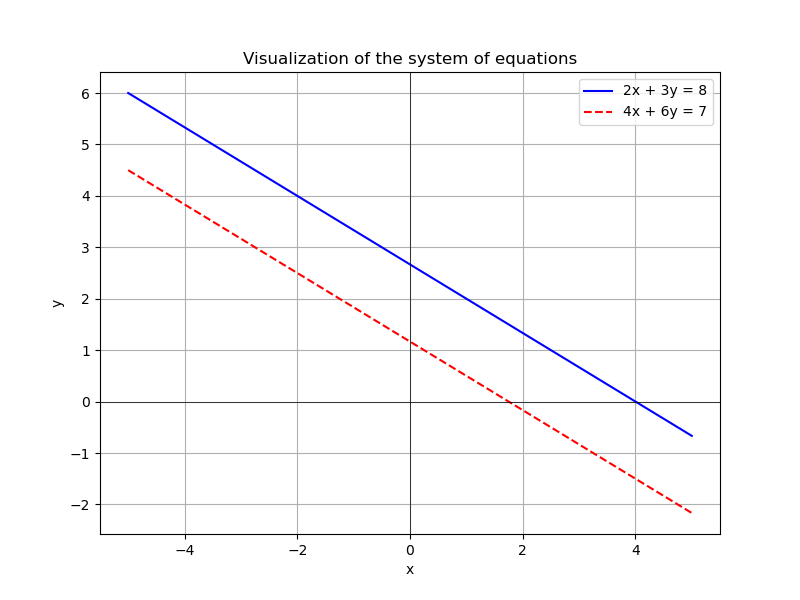
\includegraphics[width=0.6\columnwidth]{figs/fig10.png}
\end{center}
\caption{}
\label{fig:Fig}
\end{figure}    
\end{document}